% ****** Start of file template.aps ****** %
%%
%%
%%   This file is part of the APS files in the REVTeX 4 distribution.
%%   Version 4.0 of REVTeX, August 2001
%%
%%
%%   Copyright (c) 2001 The American Physical Society.
%%
%%   See the REVTeX 4 README file for restrictions and more information.
%%
%
% This is a template for producing manuscripts for use with REVTEX 4.0
% Copy this file to another name and then work on that file.
% That way, you always have this original template file to use.
%
% Group addresses by affiliation; use superscriptaddress for long
% author lists, or if there are many overlapping affiliations.
% For Phys. Rev. appearance, change preprint to twocolumn.
% Choose pra, prb, prc, prd, pre, prl, prstab, or rmp for journal
%  Add 'draft' option to mark overfull boxes with black boxes
%  Add 'showpacs' option to make PACS codes appear
%  Add 'showkeys' option to make keywords appear
% use 'preprint' or 'twocolumn' in the documentclass argument to get
% what you want
\documentclass[aps,11pt]{revtex4}
%\setlength{\topmargin}{-1.cm}{\bottommargin}{-1.cm}{\leftmargin}{-1.cm}{\rightmargin}{-1.cm}
% if you use PostScript figures in your article
% use the graphics package for simple commands
% \usepackage{graphics}
% or use the graphicx package for more complicated commands
\usepackage{graphicx}
\usepackage{color}
\pagestyle{plain}
\usepackage{hhline}
%\usepackage{colortbl}
%\usepackage[margin=2.5cm]{geometry}
% or use the epsfig package if you prefer to use the old commands
% \usepackage{epsfig}

% The amssymb package provides various useful mathematical symbols
%\usepackage{amssymb}

%\documentclass[aps,prl,preprint,superscriptaddress]{revtex4}
%\documentclass[aps,prl,twocolumn,groupedaddress]{revtex4}

% You should use BibTeX and apsrev.bst for references
% Choosing a journal automatically selects the correct APS
% BibTeX style file (bst file), so only uncomment the line
% below if necessary.
\bibliographystyle{apsrev}
\begin{document}

% Use the \preprint command to place your local institutional report
% number in the upper righthand corner of the title page in preprint mode.
% Multiple \preprint commands are allowed.
% Use the 'preprintnumbers' class option to override journal defaults
% to display numbers if necessary
%\preprint{}
%Title of paper
%\bigskip
%\hline 
%\baselineskip \baselineskip \baselineskip \baselineskip \baselineskip \baselineskip \baselineskip \baselineskip \baselineskip 
%\parskip \parskip \parskip \parskip \parskip \parskip

\title{\huge \textcolor{red}{Measurement of Nuclear Transparency for the  $A(e,e^\prime K^+)$ Reaction}}
%\hline \hline 
% repeat the \author .. \affiliation  etc. as needed
% \email, \thanks, \homepage, \altaffiliation all apply to the current
% author. Explanatory text should go in the []'s, actual e-mail
% address or url should go in the {}'s for \email and \homepage.
% Please use the appropriate macro foreach each type of information
%\renewcommand
\author{\textbf{Nuruzzaman}}
\author{\textbf{Dipangkar Dutta}}
\affiliation{Mississippi State University, Mississippi State, MS, USA}
\date{\today}
\begin{figure*}[b]
	
\includegraphics[width=0.30\textwidth]{MSU_logo.png}
	\label{fig:MSU_logo}
\end{figure*}

%\begin{turnpage}
%\collaboration{JLab K-CT collaboration}
%\noaffiliation
% \affiliation command applies to all authors since the last
% \affiliation command. The \affiliation command should follow the
% other information
% \affiliation can be followed by \email, \homepage, \thanks as well.
%\email[]{Your e-mail address}
%\homepage[]{Your ls web page}
%\thanks{}
%\altaffiliation{}

%Collaboration name if desired (requires use of superscriptaddress
%option in \documentclass). \noaffiliation is required (may also be
%used with the \author command).
%\collaboration can be followed by \email, \homepage, \thanks as well.
%\collaboration{}
%\noaffiliation
%\date{\today}
%Abstract page
\begin{abstract}
\newpage
\textbf{
\begin{center}
\Large ABSTRACT
\end{center}
}\noindent
Quantum Chromo Dynamics (QCD) is the fundamental theory of the strong force. The transition from nucleons and mesons to the quarks and gluons of QCD can be studied by looking for the onset of phenomena predicted by QCD, such as Color Transparency (CT). CT is the disappearance of final (initial) state interactions for hadrons produced in exclusive processes at high momentum transfers. An experiment to measure the transparency of pions, in search of CT was completed in Dec 2004 at JLab in Hall C. The same set of data also has a considerable sample of kaons that can be used to study the transparency of kaons. Kaon transparency via electro-production has not been studied before and will provide useful information regarding the nature of the transition from quarks to hadrons. In addition, this data will help us investigate the anomalous strangeness transparency reported for kaon-nucleus scattering data. We will extract the kaon transparency by comparing the electro-production of kaons from various nuclear targets to electro-production from hydrogen which is similar to the technique used to measure pion transparency. Preliminary results from this analysis will be presented.

%\ We have measured the nuclear transparency of the $A(e,e'K^+)$ process 
%\ in $^{2}$H,$^{12}$C, $^{27}$Al, $^{63}$Cu and $^{197}$Au targets. These measurements were performed at the Jefferson Laboratory over a four momentum transfer squared range $Q^2 = 1.1~ \mathrm{to} ~4.7~ (\mathrm{GeV/c})^2$.  The nuclear transparency was 
%\extracted as the super-ratio of $(\sigma_A/\sigma_H)$ from data to a model of pion-electroproduction from nuclei without $K^{_\_}N$ final state interactions. The $Q^2$ and atomic number dependence of the nuclear transparency both show deviations from traditional nuclear physics expectations, and are consistent with calculations that include the quantum chromodynamical phenomenon of color transparency.  

\end{abstract}
%\end{turnpage}
% insert suggested PACS numbers in braces on next line
%\pacs{25.30.Rw, 24.85.+p}
% insert suggested keywords - APS authors don't need to do this
%\keywords{}

%\maketitle must follow title, authors, abstract, \pacs, and \keywords
\maketitle
\tableofcontents
%\the content page
\newpage\textbf{\begin{center}\Large CONTENT\end{center}}

\begin{itemize}
	\item ABSTRACT\ldots\ldots\ldots\ldots\ldots\ldots\ldots\ldots\ldots\ldots\ldots\ldots\ldots\ldots\ldots\ldots\ldots\ldots\ldots2 
	\item CONTENT\ldots\ldots\ldots\ldots\ldots\ldots\ldots\ldots\ldots\ldots\ldots\ldots\ldots\ldots\ldots\ldots\ldots\ldots3
	\item LIST OF TABLES\ldots\ldots\ldots\ldots\ldots\ldots\ldots\ldots\ldots\ldots\ldots\ldots\ldots\ldots\ldots\ldots4
	\item LIST OF FIGURES\ldots\ldots\ldots\ldots\ldots\ldots\ldots\ldots\ldots\ldots\ldots\ldots\ldots\ldots\ldots\ldots\ldots5
\end{itemize}
\begin{enumerate}
	\item INTRODUCTION
	\item EXPERIMENT
	\item ANALYSIS
        \item RESULTS
	\item SUMMARY
	\item REFERNCES
        \item APPENDIX
\end{enumerate}

%\list of tables page
\newpage\textbf{\begin{center}\Large LIST OF TABLES\end{center}}

\begin{itemize}
	\item Table \ref{tab:h}: Hydrozen cross-sections and $\Sigma$ to $\lambda$ ratio
	\item Table \ref{tab:ld}: Liquid Deuterium cross-sections and Transparencies
	\item Table \ref{tab:c}: Carbon cross-sections and Transparencies
	\item Table \ref{tab:cu}: Copper cross-sections and Transparencies
	\item Table \ref{tab:g}: Gold cross-sections and Transparencies
	\item Table \ref{tab:alpha}: Alpha values for different kinematics
\end{itemize}

%\list of figures page
\newpage\textbf{\begin{center}\Large LIST OF FIGURES\end{center}}

\begin{itemize}
	\item Figure \ref{fig:HALC_33}: Hall-C of Jefferson Lab
	\item Figure \ref{fig:cointime1}: Coincedence time plot of the experiment
	\item Figure \ref{fig:cointime}: Coincedence time plot after all the cuts
	\item Figure \ref{fig:missmass}: Missingmass plot of the reaction
	\item Figure \ref{fig:pid1}: Thresolds of different hadrons for Aerogel Cherenkov
	\item Figure \ref{fig:pid2}: Thresolds of different hadrons for Gas Cherenkov
	\item Figure \ref{fig:coin_miss}: Coincedencetime Vs Missingmass plot
	\item Figure \ref{fig:missmass2}: Missingmass plot of $\lambda$, $\Sigma$ production from SIMC and Data
	\item Figure \ref{fig:missmass3}: Missingmass comparison between SIMC and Data
	\item Figure \ref{fig:Q2_1}: $Q^2$ SIMC $\lambda$, SIMC $\Sigma$ and $Q^2$ Data $\lambda$, Data $\Sigma$
	\item Figure \ref{fig:Q2_2}: $Q^2$ comparison between Data and SIMC
	\item Figure \ref{fig:w_1}: w SIMC $\lambda$, SIMC $\Sigma$ and w Data $\lambda$, Data $\Sigma$
	\item Figure \ref{fig:w_2}: w comparison between Data and SIMC
	\item Figure \ref{fig:t_1}: t SIMC $\lambda$, SIMC $\Sigma$ and t Data $\lambda$, Data $\Sigma$
	\item Figure \ref{fig:t_2}: t comparison between Data and SIMC
	\item Figure \ref{fig:phipq_1}: $\phi_{pq}$ SIMC $\lambda$, SIMC $\Sigma$ and $\phi_{pq}$ Data $\lambda$, Data $\Sigma$
  \item Figure \ref{fig:phipq_2}: $\phi_{pq}$ comparison between Data and SIMC
  \item Figure \ref{fig:transp}: Transparency Vs $Q^2$
  \item Figure \ref{fig:alpha}: $\alpha$ Vs $Q^2$
\end{itemize}

%\the introduction page
\newpage\textbf{\section{\Large Introduction}\label{sec:Introduction}}
\noindent
The nuclear transparency can be difined as
\begin{center}\textcolor{blue}{$$T=\frac{\sigma_A}{A\sigma_0}$$}\end{center}
where \textcolor{blue}{$\sigma_A$} denotes the cross-section for different targets and \textcolor{blue}{$\sigma_0$} denotes the cross-section for Hydrogen.\textcolor{blue}{$\sigma_A$} can be paramaterized in terms of free cross-sectin i.e. \textcolor{blue}{$\sigma_0$.}
\begin{center}\textcolor{blue}{$\sigma_A=\sigma_0A^\alpha$}\end{center}
Then, transparency can be written as
\begin{center}\textcolor{blue}{$$T=A^{\alpha-1}$$}\end{center}
Experimentally $\alpha$ has a value of 0.72-0.78 for different hadrons like p,K,$\pi$\\
An experiment to measure the transparency of pions, in search of CT was completed in Dec 2004 at JLab in Hall C through the elctro-production of pions by the reaction A(e,$e^\prime \pi^+$). The same set of data also has a considerable sample of kaons that can be used to study the transparency of kaons.\\
My first job was to seperate kaons from the pions and protons by applying different Particle Identification (PID).

%\the experiment page
\newpage\textbf{\section{\Large Experiment}\label{sec:Experiment}}
\noindent
We report the first measurement of the nucleon number, $A$, and $Q^2$ dependence of nuclear transparency for the process $K^+$ using the data of A(e,$e^\prime \pi^+$). The measurement was performed on $^{2}$H, $^{12}$C, $^{27}$Al, $^{63}$Cu and $^{197}$Au nuclei, over a  $Q^2$ range of 1.1 $\mathrm{to}$ 4.7 $(\mathrm{GeV/c})^2$. Measurement of both the $A$ and $Q^2$ dependence of the nuclear transparency is crucial to distinguish between CT-like effects and other reaction-mechanism based energy dependence of the transparency. In this measurement the coherence length for kaon production (distance over which the virtual photon fluctuates into a $q\bar{q}$ pair) was smaller than the nucleon radius and was essentially constant, ranging from 0.2 - 0.5 fm over the kinematic range of the experiment.

\begin{figure}[h]
	\centering
		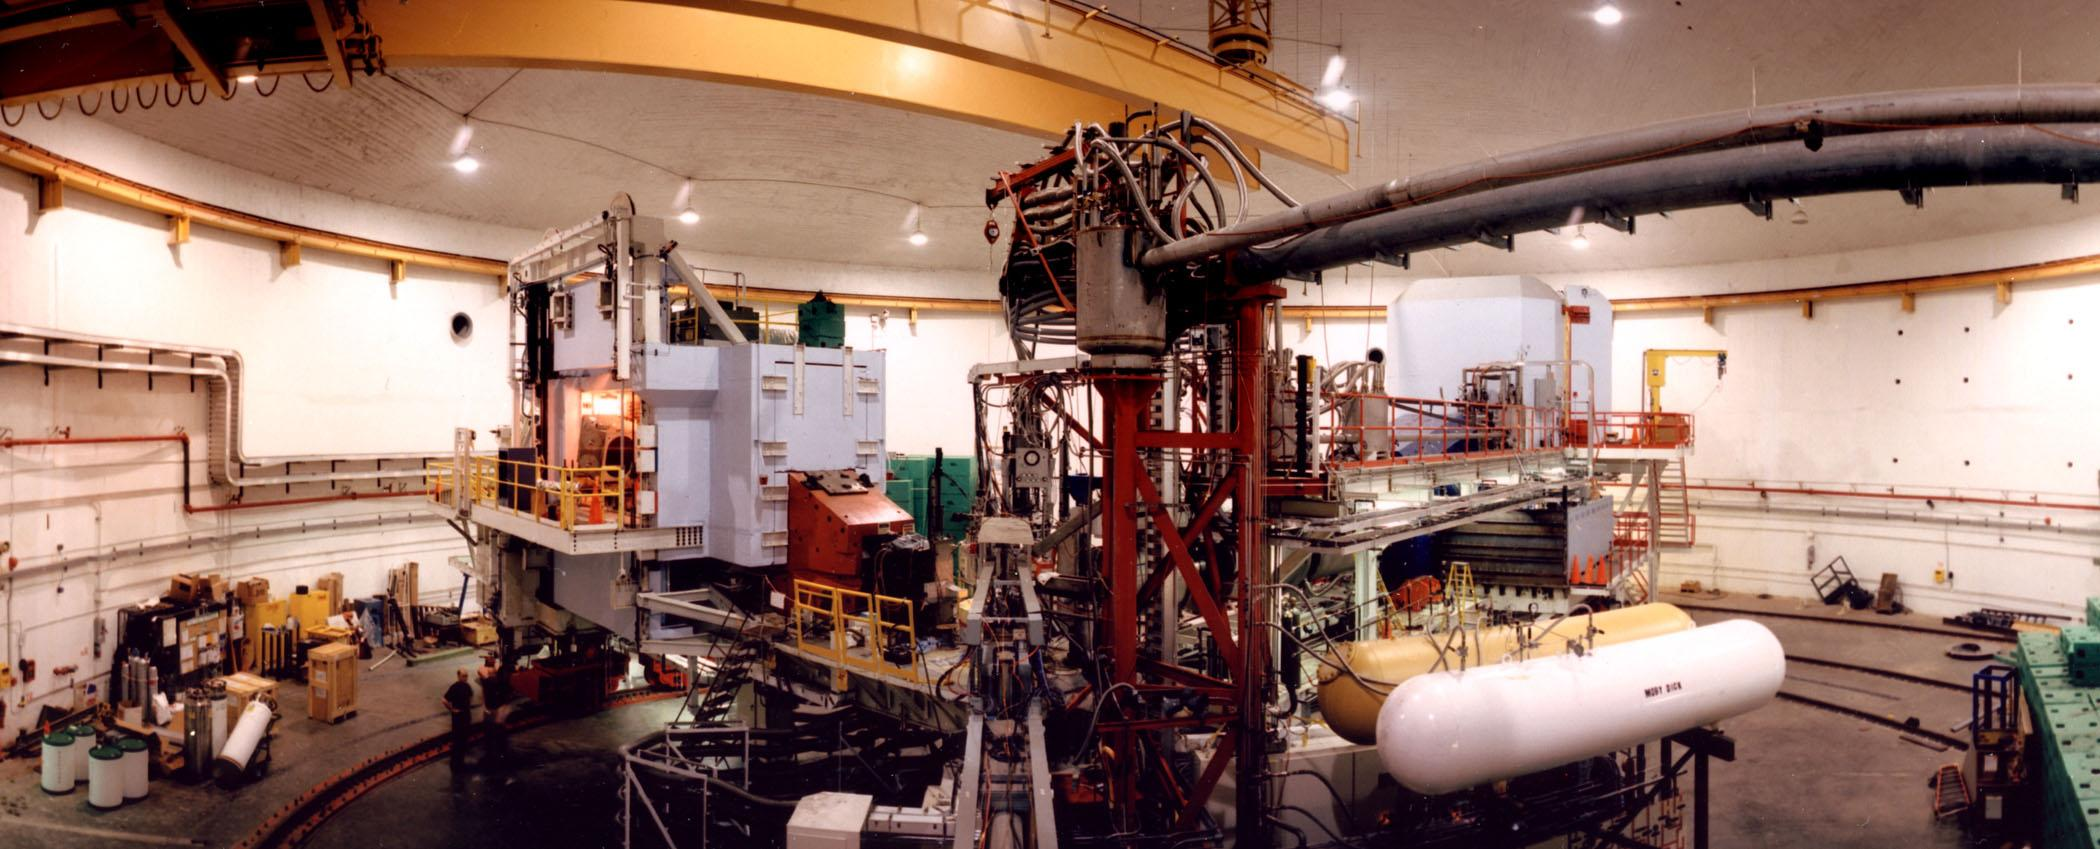
\includegraphics[width=0.40\textwidth]{HALC_33.jpg}
	\caption{Hall-C of Jefferson Lab}
	\label{fig:HALC_33}
\end{figure}

%\the analysis pages
\newpage\textbf{\section{\Large Analysis}\label{sec:Analysis}}
\noindent
If we compare our data with Monte Carlo simulation of Hall-C of Jefferson Lab named SIMC, then the nuclear transparency can be difined as:
\begin{center}\textcolor{blue}{$$T=\frac{\frac{\sigma_A}{\sigma_A^{simc}}}{\frac{\sigma_0}{\sigma_0^{simc}}}$$}\end{center}
where \textcolor{blue}{$\sigma_A^{simc}$} is the cross-section for the different targets and \textcolor{blue}{$\sigma_0^{simc}$} for Hydrozen from SIMC.

\newpage
\subsection{Coincidence Time:}
\label{sec:Coincidence Time:}
\begin{figure}[h]
	\centering
		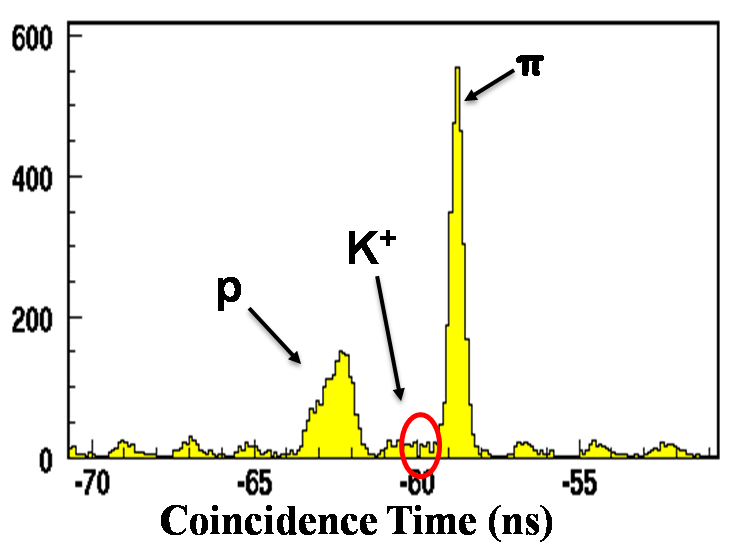
\includegraphics[width=0.40\textwidth]{cointime1.png}
	\caption{Typical coincedence time plot of the experiment}
	\label{fig:cointime1}
\end{figure}
\begin{figure}[h]
	\centering
		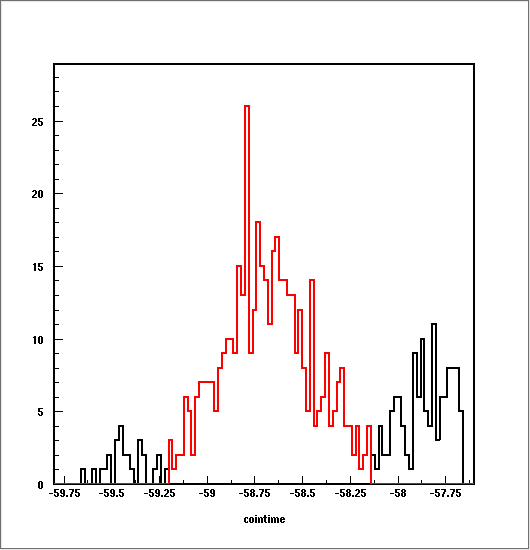
\includegraphics[width=0.40\textwidth]{cointime.png}
	\caption{Coincedence time plot after applying all the cuts for Hydrozen}
	\label{fig:cointime}
\end{figure}

\newpage
\subsection{Missing Mass:}
\label{sec:Missing Mass:}
\noindent\textbf{
Reactions:}
\begin{center}
\textcolor{blue}{
e + p $\longrightarrow$ $e^\prime$ + $K^+$ + $\lambda$ \\
e + p $\longrightarrow$ $e^\prime$ + $K^+$ + $\Sigma$
}
\end{center}
From Energy and momentum conservation calculations from the $\lambda$-channel reaction we can easily write,
\begin{center}
Energy conservation: \textcolor{blue}{$E_e$ + $M_p$ = $E_{e^\prime}$ + $E_{K^+}$ + $E_{\lambda}$} \\ 
Momentum conservation: \textcolor{blue}{$P_e$ + 0 = $P_{e^\prime}$ + $P_{K^+}$ + $P_{\lambda}$} \\
\end{center}
%\begin{minipage}[!h]{width=0.25\textwidth}
%\parabox{

\begin{figure}[!h]
\begin{flushright}
	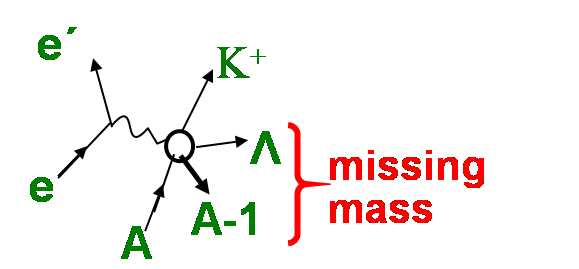
\includegraphics[width=0.40\textwidth]{reaction.png}
	\label{fig:reaction}
	\end{flushright}
\end{figure}
%\begin{minipage}[!h]{width=0.25\textwidth}
\begin{flushleft}
Then we can form a variable called \textbf{missingmass} as is 
\textcolor{blue}{$M_\lambda$ =  $[E_\lambda^2 - P_\lambda^2 ]^{1/2}$}
\end{flushleft}
%\end{minipage}

\begin{figure}[h]
	\centering
		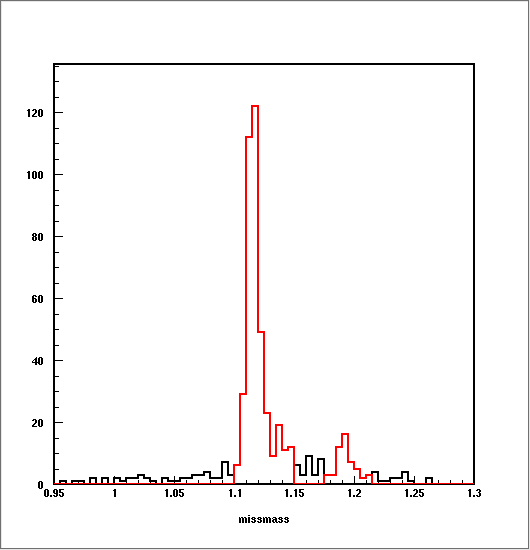
\includegraphics[width=0.40\textwidth]{missmass.png}
	\caption{Missingmass plot of the reaction}
	\label{fig:missmass}
\end{figure}
\noindent
Similarly, we can form the missingmass(\textcolor{blue}{$M_\Sigma$}) variable for $\Sigma$ production.\\
The basic idea is forming this missingmass variable and giving cuts over it in order to separate $K^+$ from p and $\pi^+$ as well as to separate $\lambda$ and $\Sigma$ production of $K^+$.

\newpage
\subsection{Cherenkov:}
\label{sec:Cherenkov:}
\begin{figure}[h]
	\centering
		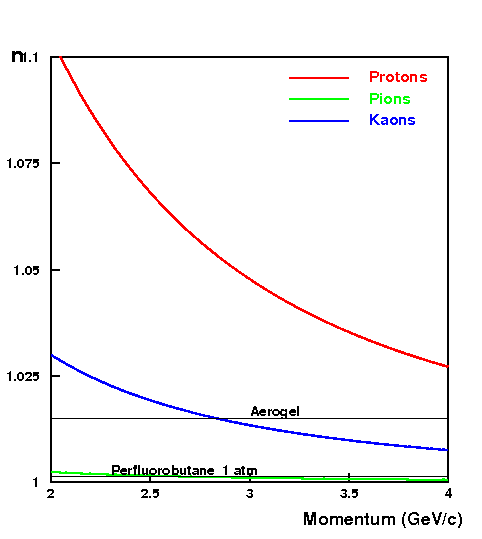
\includegraphics[width=0.40\textwidth]{pid1.png}
	\caption{Aergel cherenkov thresholds for different hadrons}
	\label{fig:pid1}
\end{figure}
\begin{figure}[h]
	\centering
		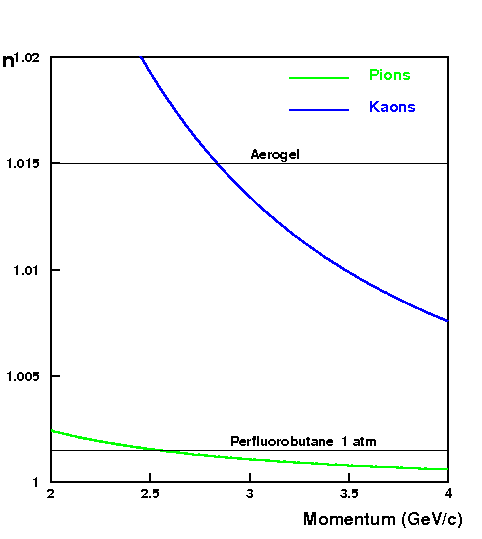
\includegraphics[width=0.40\textwidth]{pid2.png}
	\caption{Gas cherenkov thresholds for different hadrons}
	\label{fig:pid2}
\end{figure}

\newpage
\begin{figure}[h]
	\centering
		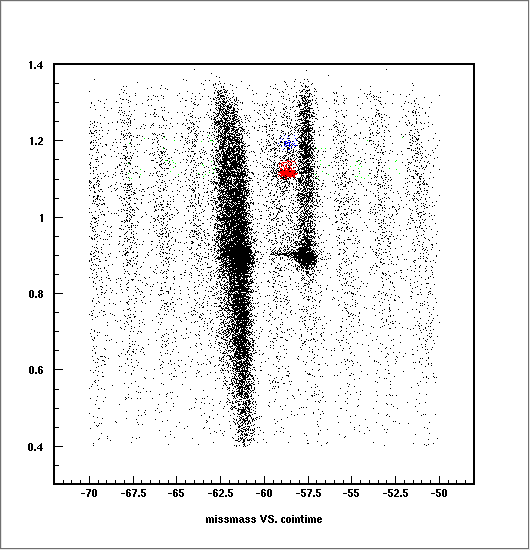
\includegraphics[width=0.40\textwidth]{coin_miss.png}
	\caption{Coincidencetime Vs Missingmass plot}
	\label{fig:coin_miss}
\end{figure}


%\the result pages
\newpage\textbf{\section{\Large Results}\label{sec:Results}}
\subsection{Basics}
\label{sec:Basics}
\noindent
The Results are shown below: 
Before determining the cross-sections ($\textcolor{blue}{\sigma}$) I have to compare the data with a simulation of Hall-C called SIMC. As $\textcolor{blue}{\sigma}$ depends on four variables i.e.\\ 
\begin{center}
$\textcolor{blue}{\sigma}$ $\equiv$  $\textcolor{blue}{\sigma}$($Q^2$, w, t, $\phi_{pq}$) where\\
\end{center}
$Q^2$$\rightarrow$ Four momentum transfers square,\\ w   $\rightarrow$ Center of mass energy,\\ t  $\rightarrow$ Mandelstam variable,\\ $\phi_{pq}$$\rightarrow$ The angle between reaction plane and scattering plane\\
Then,transparency can be difined as:
\begin{center}\textcolor{blue}{$$T=\frac{\frac{\sigma_A}{\sigma_A^{simc}}}{\frac{\sigma_0}{\sigma_0^{simc}}}$$}\end{center}
Now I need to compare data with SIMC for Hydrozen first and then for all other targets. I heve done the calculations for Hydrozen and four other different targets and for three different kinematics settings. But, here for example I will show the results for Hydrozen and Liquid Deuterium.


\newpage
\begin{figure*}[h]
	\centering
		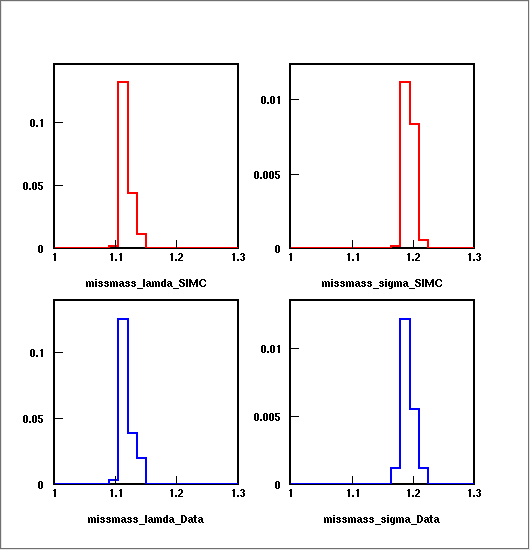
\includegraphics[width=0.40\textwidth]{missmass2.png}
	\caption{From top left to right(in \textcolor{red}{RED}) : Missingmass SIMC $\lambda$, SIMC $\Sigma$ and from bottom left to right(in \textcolor{blue}{BLUE}) : Missingmass Data $\lambda$  ,Data $\Sigma$ for Hydrozen}
	\label{fig:missmass2}
\end{figure*}
\begin{figure*}[h]
	\centering
		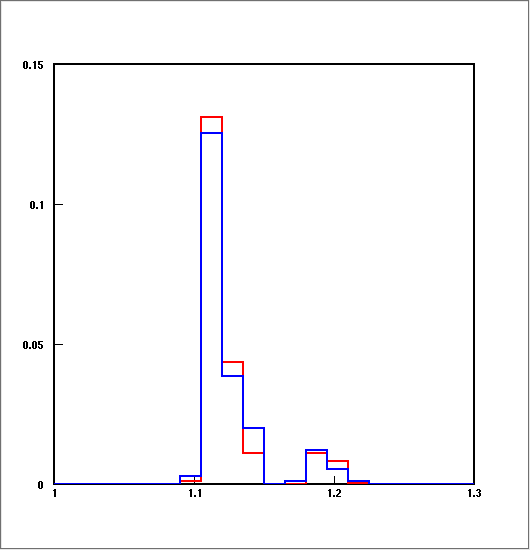
\includegraphics[width=0.40\textwidth]{missmass3.png}
	\caption{Comparison of Missingmass in SIMC(in \textcolor{red}{RED}) and Data(in \textcolor{blue}{BLUE}) for Hydrozen}
	\label{fig:missmass3}
\end{figure*}

\newpage
\subsection{The four different variables comparison between SIMC and data for Hydrozen:}
\label{sec:The four different variables comparison between SIMC and data for Hydrozen:}

\begin{figure}[h]
	\centering
%	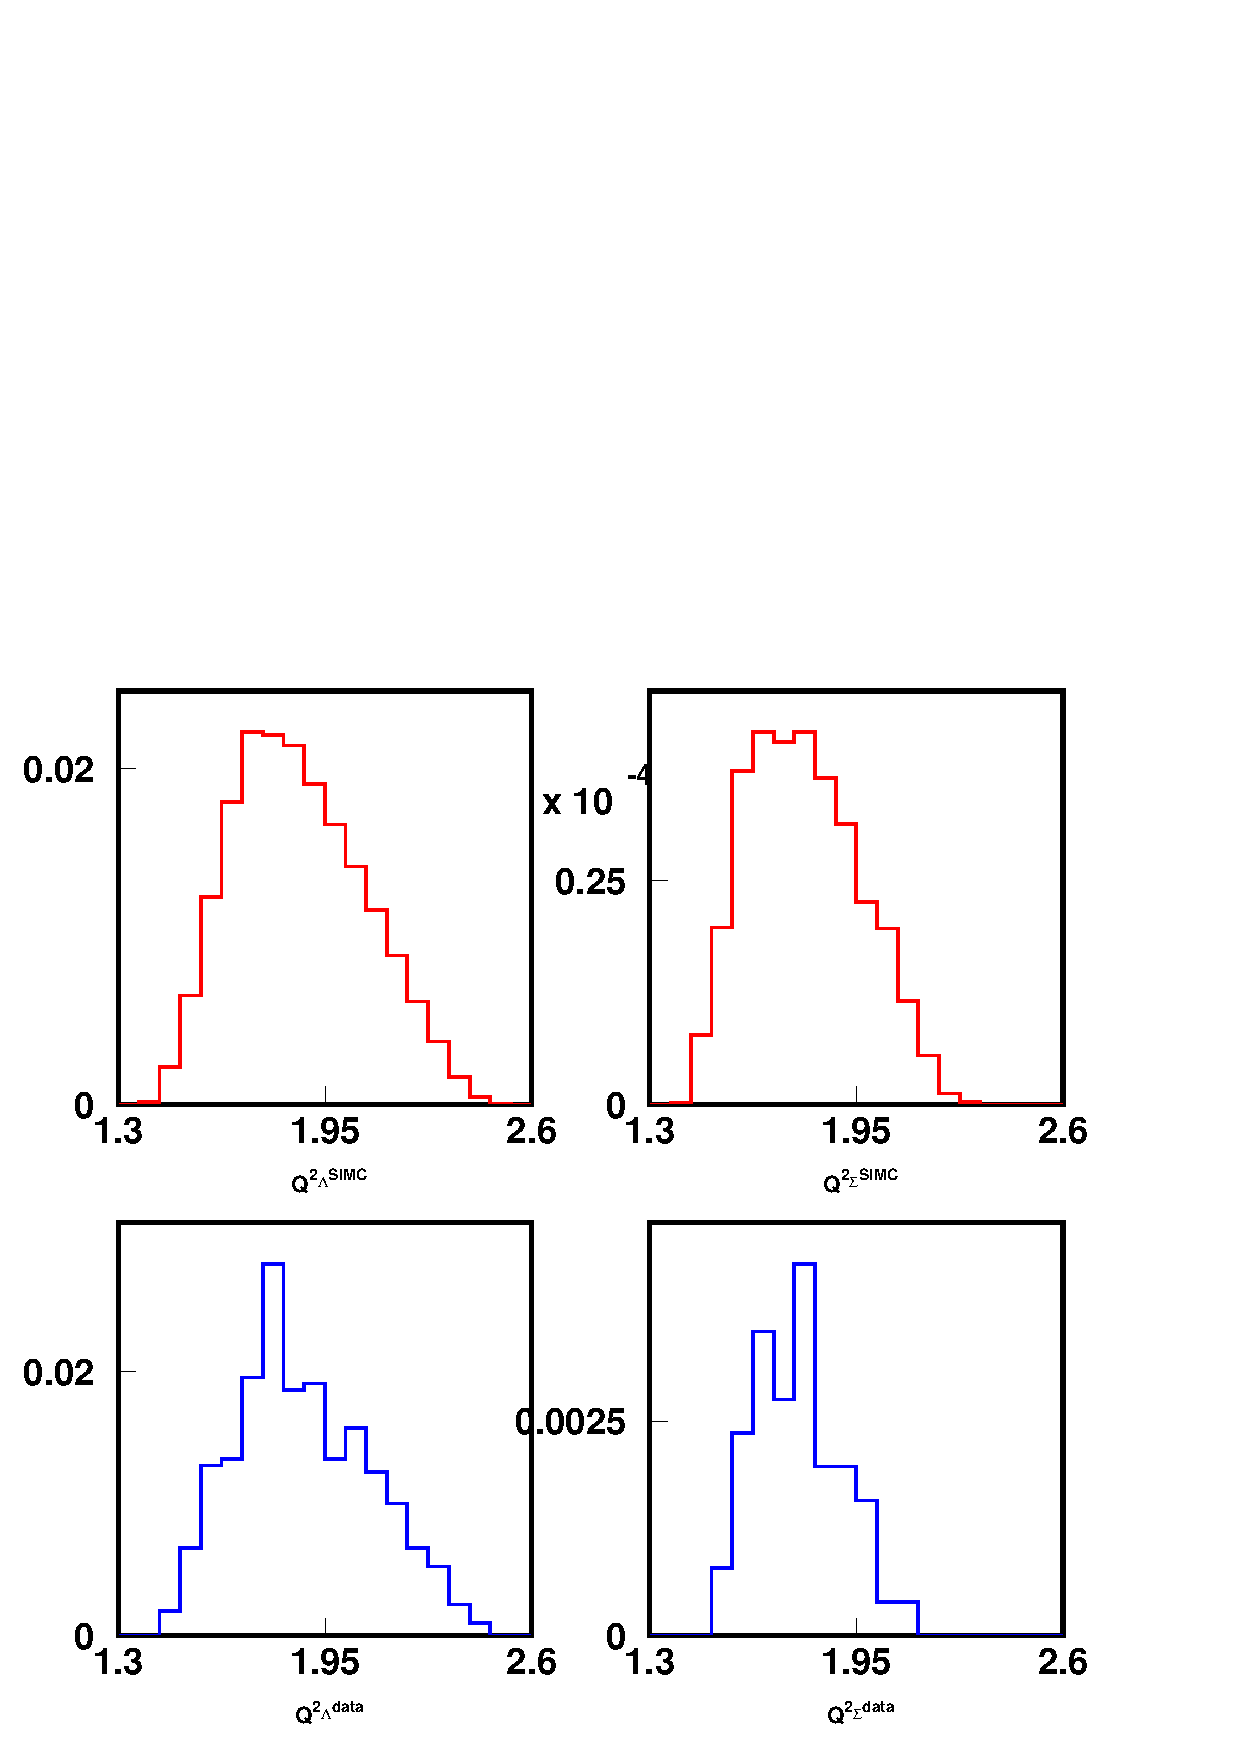
\includegraphics[width=0.40\textwidth]{Q2_1.png}
	\label{fig:Q2_1}
	\caption{From top left to right(in \textcolor{red}{RED}) : $Q^2$ SIMC $\lambda$, SIMC $\Sigma$ and from bottom left to right(in \textcolor{blue}{BLUE}) : $Q^2$ Data $\lambda$  ,Data $\Sigma$ for Hydrozen}
\end{figure}
\begin{figure}[h]
	\centering
%		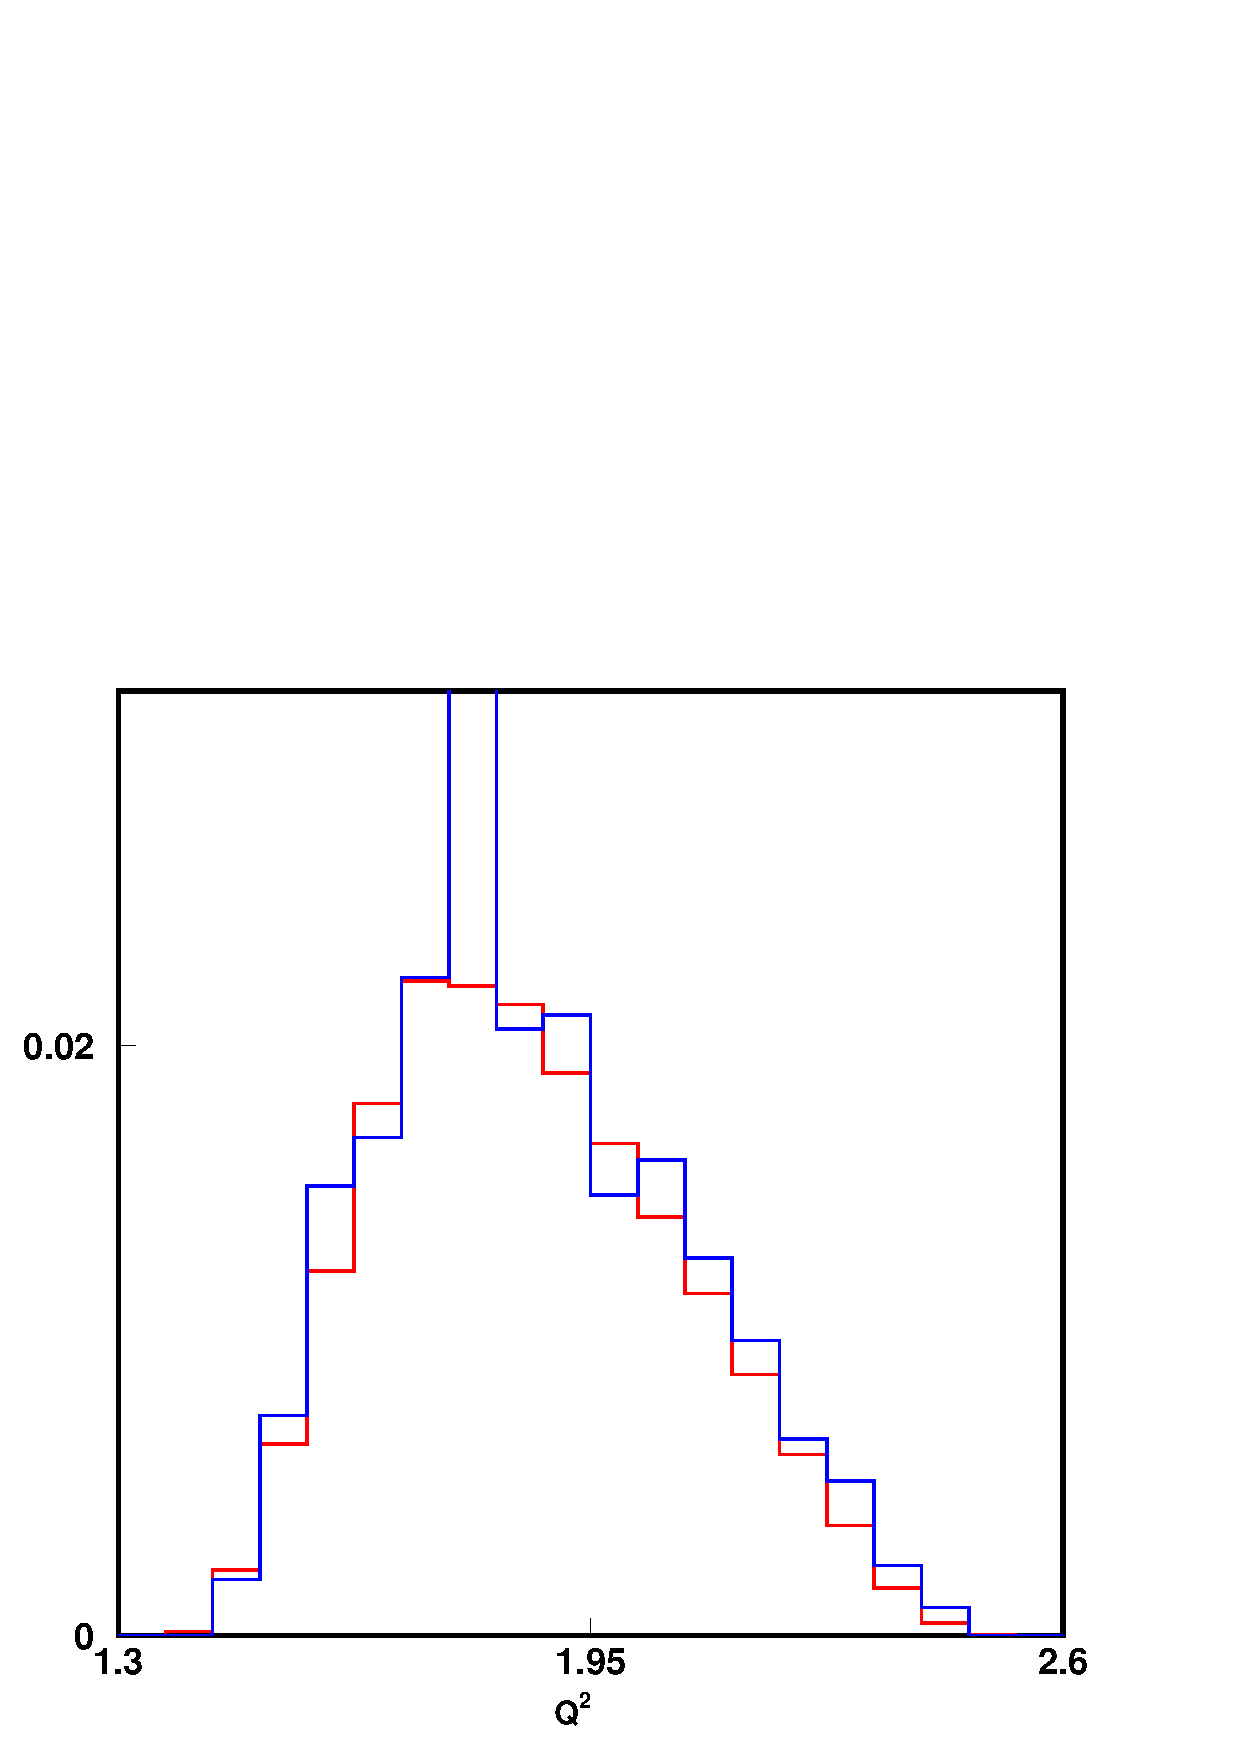
\includegraphics[width=0.40\textwidth]{Q2_2.png}
	\caption{Comparison of $Q^2$ in SIMC(in \textcolor{red}{RED}) and Data(in \textcolor{blue}{BLUE}) for Hydrozen}
	\label{fig:Q2_2}
\end{figure}
\noindent
In the \textbf{Figure \ref{fig:Q2_1}.} top left, I have shown the variable $Q^2$ from SIMC for $\lambda$-channel and top right for $\Sigma$-channel in \textcolor{red}{RED}. Then, the bottom I have shown the same for data in \textcolor{blue}{BLUE}. Basically, the ratio of $\lambda$-channel and $\Sigma$-channel has been measured by using Hydrozen data. In \textbf{Figure \ref{fig:Q2_2}.} I have added kaons for $\lambda$ and $\Sigma$ production both from SIMC shown in \textcolor{red}{RED} and data \textcolor{blue}{BLUE} with proper ratio, that I got by using Hydrozen data. The ratio of $\Sigma$ to $\lambda$ production is too small. For three kinematics i.e. for three different $Q^2$ of 1.1, 2.15, 3.0 are 0.14, 0.11, 0.09 respectively.

\newpage
\noindent
One can easily identify that the plots for different variables in the \textbf{Figures \ref{fig:Q2_2}., \ref{fig:w_2}., \ref{fig:t_2}., \ref{fig:phipq_2}.} for Hydrozen SIMC and data are matching quite well.
\begin{figure}[h]
	\centering
		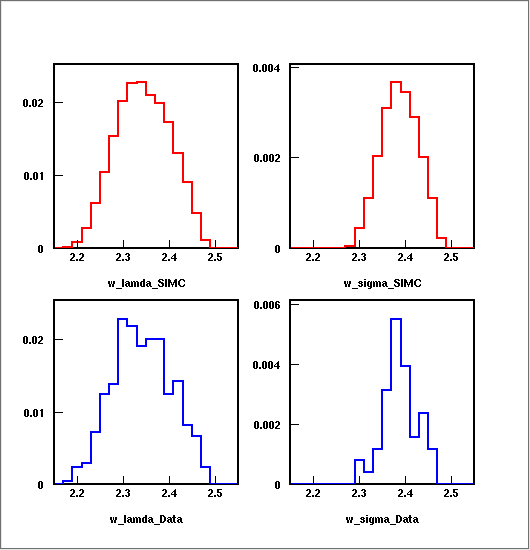
\includegraphics[width=0.40\textwidth]{w_1.png}
	\caption{From top left to right(in \textcolor{red}{RED}) : w SIMC $\lambda$, SIMC $\Sigma$ and from bottom left to right(in \textcolor{blue}{BLUE}) : w Data $\lambda$  ,Data $\Sigma$ for Hydrozen}
	\label{fig:w_1}
\end{figure}
\begin{figure}[h]
	\centering
		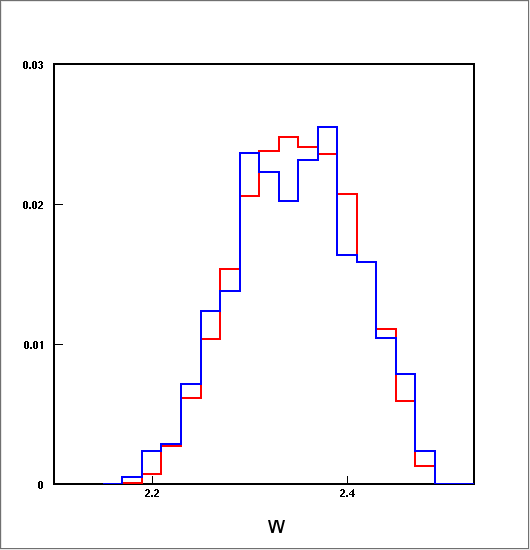
\includegraphics[width=0.40\textwidth]{w_2.png}
	\caption{Comparison of w in SIMC(in \textcolor{red}{RED}) and Data(in \textcolor{blue}{BLUE}) for Hydrozen}
	\label{fig:w_2}
\end{figure}

\newpage

\begin{figure}[h]
	\centering
		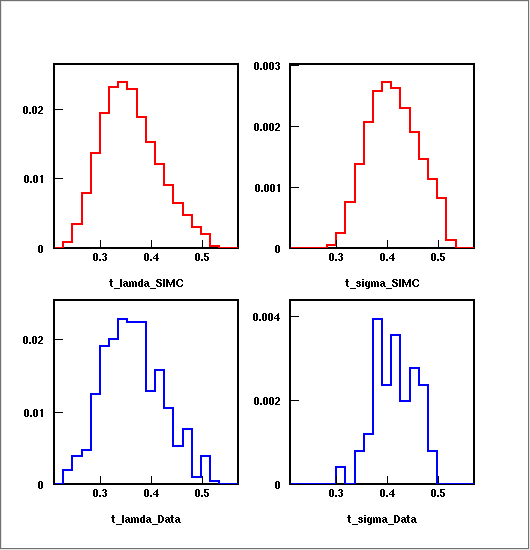
\includegraphics[width=0.40\textwidth]{t_1.png}
	\caption{From top left to right(in \textcolor{red}{RED}) : t SIMC $\lambda$, SIMC $\Sigma$ and from bottom left to right(in \textcolor{blue}{BLUE}) : t Data $\lambda$  ,Data $\Sigma$ for Hydrozen}
	\label{fig:t_1}
\end{figure}
\begin{figure}[h]
	\centering
		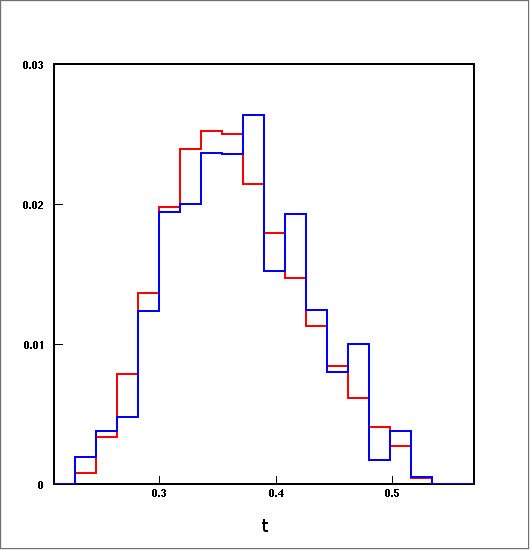
\includegraphics[width=0.40\textwidth]{t_2.png}
	\caption{Comparison of t in SIMC(in \textcolor{red}{RED}) and Data(in \textcolor{blue}{BLUE}) for Hydrozen}
	\label{fig:t_2}
\end{figure}

\newpage

\begin{figure}[h]
	\centering
		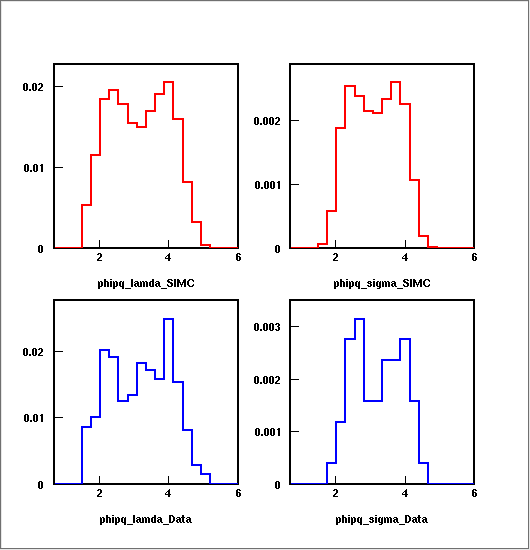
\includegraphics[width=0.40\textwidth]{phipq_1.png}
	\caption{From top left to right(in \textcolor{red}{RED}) : $\phi_{pq}$ SIMC $\lambda$, SIMC $\Sigma$ and from bottom left to right(in \textcolor{blue}{BLUE}) : $\phi_{pq}$ Data $\lambda$  ,Data $\Sigma$ for Hydrozen}
	\label{fig:phipq_1}
\end{figure}
\begin{figure}[h]
	\centering
		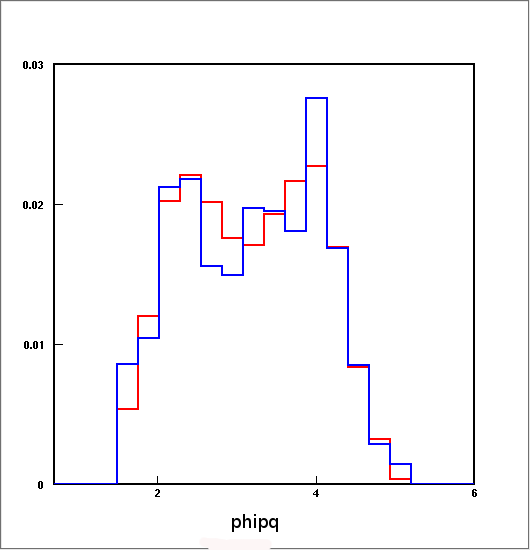
\includegraphics[width=0.40\textwidth]{phipq_2.png}
	\caption{Comparison of $\phi_{pq}$ in SIMC(in \textcolor{red}{RED}) and Data(in \textcolor{blue}{BLUE}) for Hydrozen}
	\label{fig:phipq_2}
\end{figure}

\newpage
\subsection{The four different variables comparison between SIMC and data for Liquid Deuterium:}
\label{sec:The four different variables comparison between SIMC and data for Liquid Deuterium:}

\newpage
\subsection{The nuclear transparency for different targets}
\label{sec:The nuclear transparency for different targets}

\begin{figure*}[h]
	\centering
		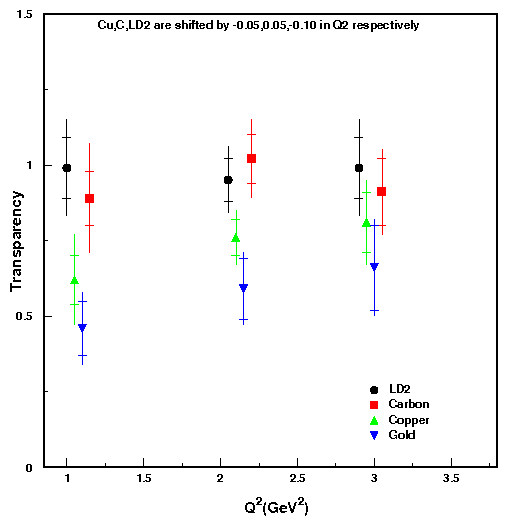
\includegraphics[width=0.40\textwidth]{transp.png}
	\caption{Transparency Vs $Q^2$}
	\label{fig:transp}
\end{figure*}

\begin{table}[!ht] 
%\begin{ruledtabular}
%\colorbox{green}{
\begin{tabular}{||c|c|c|c|c|c||}\hline
 $Q^2$ & $\Sigma$ to $\lambda$ Ratio & Hydrozen Crossection & Statistical Uncertinity & Systematic Uncertinity & Total Uncertinity \\
 (GeV/c)$^2$ & & mb & $\%$ & $\%$ & $\%$ \\\hline
1.10 &0.14 &9.46 &6.28 &5.61 &8.42 \\
2.15 &0.11 &8.72 &4.76 &4.41 &6.49 \\
3.00 &0.09 &9.29 &7.44 &4.89 &8.91 \\\hline      
\end{tabular}
\caption{\label{table1} The cross-sections of Hydrozen for different kinematics.}\label{tab:h}
%}
%\end{ruledtabular}  
\vspace{-0.5cm}
\end{table}

\begin{table}[!ht] 
%\begin{ruledtabular}
%\colorbox{green}{
\begin{tabular}{||c|c|c|c|c|c||}\hline
 $Q^2$ & $LD_2$ Crossection & Statistical Uncertinity & Systematic Uncertinity & Total Uncertinity & Transparency \\
 (GeV/c)$^2$ & mb & $\%$ & $\%$ & $\%$ &  \\\hline
1.10 &8.38 &10.30 &12.34 &16.07 &0.88 \\
2.15 &7.53 &07.51 &07.48 &10.61 &0.86  \\
3.00 &8.55 &10.22 &12.06 &15.81 &0.92 \\\hline      
\end{tabular}
\caption{\label{table1} The cross-sections and transparencies of Liquid Deuterium for different kinematics.}\label{tab:ld}
%}
%\end{ruledtabular}  
\vspace{-0.5cm}
\end{table}

\begin{table}[!ht] 
%\begin{ruledtabular}
%\colorbox{green}{
\begin{tabular}{||c|c|c|c|c|c||}\hline
 $Q^2$ & Carbon Crossection & Statistical Uncertinity & Systematic Uncertinity & Total Uncertinity & Transparency \\
 (GeV/c)$^2$ & mb & $\%$ & $\%$ & $\%$ &  \\\hline
1.10 &7.57 &09.31 &16.11 &18.61 &0.80 \\
2.15 &8.01 &07.58 &10.03 &12.57 &0.91 \\
3.00 &7.76 &11.49 &08.10 &14.06 &0.84 \\\hline      
\end{tabular}
\caption{\label{table1} The cross-sections and transparencies of Carbon for different kinematics.}\label{tab:c}
%}
%\end{ruledtabular}  
\vspace{-0.5cm}
\end{table}

\begin{table}[!ht] 
%\begin{ruledtabular}
%\colorbox{green}{
\begin{tabular}{||c|c|c|c|c|c||}\hline
 $Q^2$ & Copper Crossection & Statistical Uncertinity & Systematic Uncertinity & Total Uncertinity & Transparency \\
 (GeV/c)$^2$ & mb & $\%$ & $\%$ & $\%$ &  \\\hline
1.10 &5.17 &07.85 &12.69 &14.92 &0.55 \\
2.15 &5.61 &06.45 &06.43 &09.11 &0.64 \\
3.00 &6.75 &10.24 &09.33 &13.85 &0.73 \\\hline      
\end{tabular}
\caption{\label{table1} The cross-sections and transparencies of Copper for different kinematics.}\label{tab:cu}
%}
%\end{ruledtabular}  
\vspace{-0.5cm}
\end{table}

\begin{table}[!ht]
%\begin{ruledtabular}
%\colorbox{green}{
\begin{tabular}{||c|c|c|c|c|c||}\hline
 $Q^2$ & Gold Crossection & Statistical Uncertinity & Systematic Uncertinity & Total Uncertinity & Transparency \\
 (GeV/c)$^2$ & mb & $\%$ & $\%$ & $\%$ &  \\\hline
1.10 &3.64 &09.03 &07.13 &11.51 &0.39 \\
2.15 &4.49 &09.93 &06.40 &11.82 &0.51 \\
3.00 &5.42 &13.91 &08.22 &16.16 &0.58 \\\hline      
\end{tabular}
\caption{\label{table1} The cross-sections and transparencies of Gold for different kinematics.}\label{tab:g}
%}
%\end{ruledtabular}  
\vspace{-0.5cm}
\end{table}

\begin{figure*}[!ht]
	\centering
		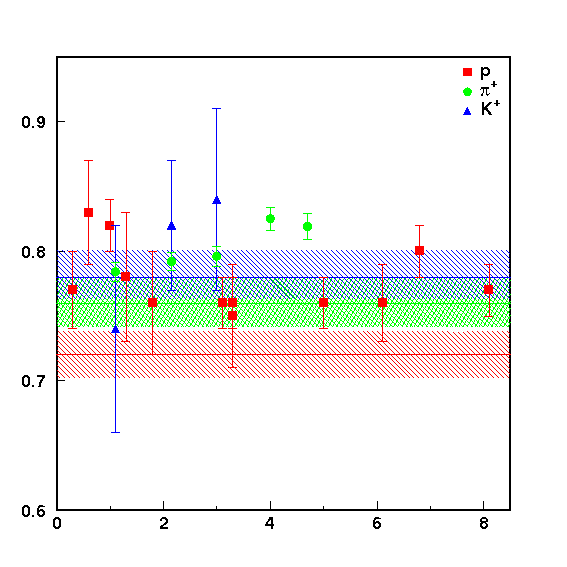
\includegraphics[width=0.40\textwidth]{alpha.png}
	\caption{Alpha Vs $Q^2$}
	\label{fig:alpha}
\end{figure*}

\begin{table}[!ht] 
%\begin{ruledtabular}
%\colorbox{green}{
\begin{tabular}{||c|c|c||}\hline
 $Q^2$ & $\alpha$ & Uncertinity \\
 (GeV/c)$^2$ &  & $\%$ \\\hline
1.10 & 0.84 &6.0 \\
2.15 & 0.91 &4.0 \\
3.00 & 0.92 &5.0 \\\hline
\end{tabular}
\caption{\label{table1} $\alpha$ for different kinematics with theoritical band.}\label{tab:alpha}

%}
%\end{ruledtabular}  
\vspace{-0.5cm}
\end{table}


\newpage
%In the context of perturbative Quantum Chromo Dynamics (QCD), Brodsky and Mueller~\cite{Mueller:1982} predicted that at sufficiently high momentum transfers, the quark-gluon wave packets of hadrons can be produced as a `color neutral' object of a reduced transverse size. If this compact size is maintained for some distance in traversing the nuclear medium, it would pass undisturbed through the nuclear medium. This is the so-called phenomenon of color transparency (CT). Nuclear transparency, defined as the ratio of the cross section per nucleon 
%for a process on a bound nucleon in the nucleus to that from a free nucleon, is the observable used to search for CT. 
%A clear signature for the onset of CT would involve a rise in the 
%nuclear transparency as a function of $Q^2$. Later works 
%\cite{CTreview} have indicated that this phenomenon also occurs 
%in a wide variety of models which feature non-perturbative reaction
%mechanisms. 
%
%More recently, CT has been discussed in the context of a QCD factorization
%theorem derived for meson electroproduction~\cite{factor1}, which states that the meson production amplitude can be expressed in terms of a hard scattering process, a distribution amplitude for the final state meson and a parametrization of the non-perturbative physics inside the nucleon known as Generalized Parton Distributions (GPDs)~\cite{gpd1}. Factorization is expected to be valid for $Q^2 \ge$ 10 (GeV/c)$^2$, however, under certain conditions it may also be applicable at lower $Q^2$~\cite{factor3}. It has been suggested that the onset of CT is a necessary (but not sufficient) condition for factorization to occur~\cite{strikman}. The underlying assumption is that in exclusive ``quasielastic'' production,  the hadron is produced at small inter-quark distances. Thus, the unambiguous observation of the onset of CT is critical as a precondition to the validity of factorization in meson production, and because it would open a new window to study the strong interaction in nuclei. 
%
%
%A number of searches for CT have been carried out in experiments using the $A(p,2p)$, $A(e,e'p)$ reactions, coherent and incoherent meson production from nuclei and kaon photoproduction reactions~\cite{ct6}~--~\cite{gammapi}. At high energies the di-jet experiment at Fermi Lab~\cite{fermipi} and $\rho^0$ production at DESY~\cite{hermesrho} are consistent with CT, and it is necessary to include CT to understand shadowing in nuclear deep inelastic scattering~\cite{ff94}. However, the predicted onset of CT at intermediate energies, typical of experiments at JLab and BNL, has not yet been unambiguously observed.  The most recent experiment at JLab to look for CT in $qqq$ hadrons using the $A(e,e'p)$ reaction~\cite{hallc_ct}, does not show any increase of the nuclear transparency up to $Q^2$ = 8.1 (GeV/c)$^2$ and rules out several models predicting an early, rapid onset of CT. One should expect an earlier onset of CT for meson production than for proton scattering~\cite{blattel93}, as it is much more probable to produce a small transverse size in a $q\bar{q}$ system than in a $qqq$ system. Moreover, the 
%evolution distances are easily longer than the nuclear radius~\cite{CTreview}, even at moderate $Q^2$, which increases the chances for the small transverse size object to pass undisturbed through the nucleus. These arguments seem to be supported by a recent kaon-photoproduction experiment at JLab~\cite{gammapi}. 
%%CT at Jlab energies is important
%%because its existence would be relevant to understand the nuclear EMC effect and possible medium modification of the electromagnetic form factors of bound nucleons. 
%%These ideas are 
%%supported by several experiments performed at Fermi Lab, DESY and most 
%%recently at JLab~\cite{fermipi}~--~\cite{gammapi}.  Unambiguous observation of CT would provide a new window to study the strong interaction in nuclei.
%
%
%%In this letter, 
%We report the first measurement of the nucleon number, $A$, and $Q^2$ dependence of nuclear transparency for the $A(e,e'K^+)$ process. The measurement was performed on $^{2}$H, $^{12}$C, $^{27}$Al, $^{63}$Cu and $^{197}$Au nuclei, over a  $Q^2$ range of 1.1 $\mathrm{to}$ 4.7 $(\mathrm{GeV/c})^2$. Measurement of both the $A$ and $Q^2$ dependence of the nuclear transparency is crucial to distinguish between CT-like effects and other reaction-mechanism based energy dependence of the transparency. In this measurement the coherence length for pion production (distance over which the virtual photon fluctuates into a $q\bar{q}$ pair) was smaller than the nucleon radius and was essentially constant, ranging from 0.2 - 0.5 fm over the kinematic range of the experiment.   
%
%%***Description of the experiment***
%
%An experiment was performed in Hall-C at JLab over the summer and fall of 2004 for measurement of pion transparency. The experiment was basically disigned for measurement of pion transparency; but, in that coincidence window of pion some kaons were also produced during the reaction. I have extracted kaon transparency using the data of that experiment. In that experiment a continuous wave electron beam with energies between 4 and 5.8~GeV and currents between 10 and 80 $\mu$A was incident on solid foil targets of $^{12}$C, $^{27}$Al, $^{63}$Cu and $^{197}$Au, and 4~cm long liquid hydrogen and deuterium targets. The $^{27}$Al target was used to mimic the cell walls of the liquid target, and enabled the events from the walls to be subtracted from the hydrogen and deuterium data. The scattered electrons and the electroproduced kaons ($K^+$) were detected in coincidence using the Short Orbit Spectrometer (SOS) and the High Momentum Spectrometer (HMS) respectively. The kinematic settings of the measurements are shown in Table ~\ref{table1}. The center of mass energy of the hadron system, $W$, for all these settings was above 2.14 GeV in order to avoid the resonance region. In addition to the kinematics shown in Table~\ref{table1}, data were collected using the hydrogen target over a range of $\pm$ 5$^o$ around the momentum transfer direction, $\theta_{q} = \theta_{k}$, for each $Q^2$ setting (except when limited by the hardware constraint $\theta_{\rm HMS}>$ 10.6$^{\circ}$). These data helped 
%develop a model of the elementary kaon electroproduction cross section covering a greater range in $\theta_q$. For two $Q^2$ settings (2.15 and 3.91 (GeV/c)$^2$) data were also collected at a larger electron scattering angle, in order to perform a Rosenbluth separation as a check of the reaction mechanism. The results of the Rosenbluth separation will be presented in a forthcoming article. 
%\begin{table}
%\caption{\label{table1} The central kinematics of the experiment.}
%%\begin{ruledtabular}
%\colorbox{green}{
%\begin{tabular}{|c|c|c|c|c|c|c|c|}\hline
% $Q^2$ & $-t$ & $E_e$ & $\theta_{e^\prime}^{\rm SOS}$ &$E_{e^\prime}$ &
% $\theta_{k}$ & $\theta_{\rm HMS}$ & $p_k$ \\
% (GeV/c)$^2$ & (GeV/c)$^2$ & GeV & deg & GeV & deg & deg & GeV/c \\\hline
%1.10 &0.050 &4.021 &27.76 &1.190 &10.58 &10.61 &2.793 \\
%2.15 &0.158 &5.012 &28.85 &1.730 &13.44 &13.44 &3.187 \\
%3.00 &0.289 &5.012 &37.77 &1.430 &12.74 &12.74 &3.418 \\
%3.91 &0.413 &5.767 &40.38 &1.423 &11.53 &11.53 &4.077 \\
%4.69 &0.527 &5.767 &52.67 &1.034 & 9.09 &10.63 &4.412 \\\hline      
%\end{tabular}}
%%\end{ruledtabular}  
%\vspace{-0.5cm}
%\end{table}
%
%The SOS gas \v{C}erenkov counter was used to select the scattered electrons with an efficiency of better than 99.2\%. The kaons were selected using the HMS  aerogel~\cite{aerogel} and gas \v{C}erenkov counters, with better than 98.8\% and 99.1\% efficiency, respectively. The HMS aerogel \v{C}erenkov counter was used to select kaons only for HMS central momenta $<$~3.2~(GeV/c), because they were below the pion threshold in the HMS gas \v{C}erenkov counter. At higher momentum settings, the HMS gas \v{C}erenkov counter alone was sufficient for selecting kaons. The spectrometer acceptance was determined with a relative uncertainty of 1\% between targets using a Monte Carlo simulation of the experimental apparatus, as described below. For each run, the $e-K^+$ coincidence events were corrected for random coincidences. %which were typically less than 25\% of the events. 
%The charge weighted coincidence yield was also corrected for blocked coincidences ($< $ 0.7\%), loss of synchronization between detectors ($< $ 1.0\%), trigger inefficiency ( $< $ 0.5\%), electronic dead time ( $< $ 1.0\%), computer dead time ( $< $ 25\%, known to much better than 1\%), tracking inefficiency ( $< $ 4.0\%) and particle absorption in the spectrometer material (5.0\% known to better than 0.5\%).  Events from multiple-kaon production were rejected with a cut on the missing mass spectrum for each target. Using a simulation of the multiple-pion background it was estimated that the contamination from such events was $<$ 0.4\%. 
%
%%***Simulation***
%The standard Hall C Monte Carlo simulation code SIMC was used to simulate the experimental apparatus~\cite{ben_thesis}. 
%%A quasi-free reaction mechanism was assumed for the $A(e,e'K^+)$ process. 
%The $p(e,e'K^+)n$ cross section needed in the model was iterated until 
%there was good agreement between the simulation and the experimental data. The iteration was performed separately for each of the kinematic settings in Table ~\ref{table1}. A parametrization of the $p(e,e'K^+)n$ cross section from previous data~\cite{tanja_thesis} was used as the 
%starting model. 
%
%%\begin{figure}
%%\begin{center}
%%\includegraphics[width=75mm, height=70mm]{prl0.eps}
%%\caption[]{The missing-mass spectra for $^{12}C(e,e'\pi)$; the crosses are data, the solid line is the simulation which is normalized to the data. The shaded region shows the simulated multi-pion background. The vertical line indicates the position of the multi-pion cut as defined in the text. }
%%\label{eepi_dist}
%%\vspace{-1.0cm}
%%\end{center}
%%\end{figure}
%
%The Fermi motion of the nucleons in $A>1$ targets was simulated by folding the elementary cross section with a spectral function for the target. For each target, an appropriate Independent Particle Shell Model (IPSM) spectral function was used~\cite{013longpaper}. 
%%When tested with non-IPSM spectral functions the model yields for a $^{12}$C 
%%target changed by $\sim$ 4\% and had an energy dependence of $\pm$1\%. 
%The simulation includes several corrections such as kaon decay within the spectrometer, external and internal bremsstrahlung radiation and kaons punching through the collimators at the spectrometer entrance. It also included corrections due to various reaction mechanism of the $A(e,e'K^+)$ process such as the Coulomb distortion of the incoming and scattered electrons, the bound proton in the target nuclei being off-shell and Pauli exclusion of the recoiling neutron. 
%%%%%%The separation energy for the bound proton was set to zero in order to best reproduce the effects of the bound proton being off-shell. Pauli blocking was simulated using nucleon distribution functions obtained from Ref.~\cite{fantoni}. 
%
%%Multiple-pion production was also included in the simulation. 
%The phase space for multiple-kaon production within the spectrometer acceptance was simulated assuming a quasi-free single kaon production and a uniform phase space distribution of the additional kaons. The simulated multi-kaon strength was normalized to the tail of the experimental missing mass spectra. The multiple-kaon simulation was used to determine the location of the cut 
%on the experimental missing mass spectrum such that the contamination from 
%multiple-kaon events was less than 0.4\%. This allowed the missing mass cut to be 
%placed $\sim$ 10 -- 50 MeV/c$^2$ above the actual kinematic threshold for two-kaon production. The simulation 
%was able to reproduce the shapes of the measured $W$, $Q^2$ and $|t|$ distributions versus the missing mass reasonably well for all targets and $Q^2$ settings.  Representative missing-mass spectra for $^{12}C(e,e'K)$ are shown
%together with the Plane Wave Impulse Approximation (PWIA) simulation in Fig.~\ref{eepi_dist} for
%all $Q^2$ settings. 
%%The vertical dashed line is the location of the cut used to reject
%%multiple-pion events. 
%The agreement between the missing mass spectra obtained from data and 
%simulation improve with increasing $Q^2$. The discrepancy seen at $Q^2$ = 1.1 (GeV/c)$^2$ can be attributed to the reaction mechanisms missing from the simulations such as final state interactions between the knocked-out neutron and the residual nucleons (nN-FSI) and short range correlations. 
%
%In order to extract the nuclear transparency from the experimental yields, 
%the cross section for the bound proton must be corrected for the effects of Fermi motion, Pauli blocking, the off-shell properties of the proton and the acceptances of the spectrometers. In order to account for these 
%effects, the nuclear transparency was formed using the experimental charge normalized yield, $\bar Y$, divided by the charge normalized Monte Carlo equivalent yield, $\bar Y_{\rm MC}$. For a given target,
%with nucleon number, $A$, the nuclear transparency was defined as:
%\begin{equation} \label{equ:nucltransp}
%T = 
%{\left( \bar Y/ \bar Y_{\rm MC} \right)_A} /
%{\left( \bar Y/ \bar Y_{\rm MC} \right)_{\rm H}},
%\end{equation}
%where the denominator is the ratio of the yields from the $^1$H target.
%As the Monte Carlo simulation does not include final-state interactions between the kaon and the residual nucleons, the nuclear transparency is a measure of these final-state interactions, and the reduction of these interactions is a signature of CT. 
%
%  
%%\begin{figure}
%%\begin{center}
%%\includegraphics[width=75mm,height=55mm]{prl1.eps}
%%\caption
%%{Nuclear transparency, T, vs. $Q^2$ for $^2$H and $^{12}$C (left, top panel), $^{27}$Al (right, top), $^{63}$Cu (left, bottom) and  $^{197}$Au (right, bottom). The inner error bars are the statistical uncertainties and the outer error
%%bars are the statistical and point-to-point systematic uncertainties added in
%%quadrature. The dark band in the bottom right panel is the $Q^2$ dependent model uncertainty, and is the same for all nuclei. The solid and dashed lines are Glauber and Glauber plus CT calculations, respectively~\cite{Larson06ge}. 
%%The solid lines are Glauber type calculations and the
%%dashed lines are Glauber plus CT (both sets of calculations are from Refs.~\cite{Larson06ge,Larson_priv}). 
%%The CT calculation assumed $\Delta M^2=0.7$~(GeV/c$^2$)$^2$. 
%%Similarly, the dot-dash and dotted lines are Glauber and Glauber plus CT calculations, respectively~\cite{wim}. These calculations also include the effect of short range correlations (SRC). 
%%All curves have been normalized to pass through the lowest Q$^2$ point. 
%%the normalization factors for the curves from Ref~\cite{kundu} are 1.13, 1.37 and 1.25, respectively for $^{12}$C, $^{63}$Cu and $^{197}$Au. 
%%}  
%
%%\label{fig1}
%%\vspace{-1.0cm}
%%\end{center}
%%\end{figure}
%%\vspace{0.5cm}
%
%Traditional nuclear physics calculations based on the Glauber multiple
%scattering mechanism~\cite{glauber} are expected to be energy-independent ( because the $K$-nucleon cross section is constant for the energies in this experiment).  To investigate the energy dependence, the extracted 
%nuclear transparency is shown as a function of $Q^2$ in
%Fig.~\ref{fig1}. The point-to-point ($Q^2$ dependent) systematic uncertainty is 2.4 -- 3.2\%, dominated by uncertainty in the spectral function (1\%) and the iteration procedure (1\%). There is an additional normalization systematic uncertainty of 1.1\% (not shown in the figure) with pion absorption correction (0.5\%), and target thickness (1\%) being the main sources. The $Q^2$ dependent model uncertainty is 7.6\%, 5.7\%, 3.5\%, 3.8\% and 3.8\% for $Q^2$ = 1.1, 2.1, 3.0, 3.9 and 4.7 (GeV/c)$^2$ respectively. This uncertainty was determined from the change in $Q^2$ dependence of the transparency when using two different spectral functions and two different Fermi distributions in the simulation, and the $Q^2$ dependent uncertainty from reactions mechanisms not included in the simulation (estimated by quantifying the difference in shape of the missing-mass spectra from data and simulation) added in quadrature. The $Q^2$ dependent model uncertainty is shown as a dark band in the bottom right panel of Fig.~\ref{fig1}. There is an additional 7.0\% normalization type model uncertainty, independent of $Q^2$, not shown in the figure.
%The observed $Q^2$ dependence of the transparency deviates from the 
%calculations without CT of Larson {\it et al.} and Cosyn {\it et al.}~\cite{Larson06ge,wim}, and are in better 
%agreement with the CT calculations of the same authors. Larson {\it et al.} use a semi-classical Glauber multiple scattering approximation, while Cosyn {\it et al.} use a relativistic version of Glauber multiple scattering theory. Both groups incorporate CT using the quantum diffusion model of Ref.~\cite{farrar} with the same parameters $\tau$ = 1~fm/c and $M_h^2$ = 0.7 GeV$^2$. 
% 
%
%In addition to the $Q^2$ dependence,
%the dependence of the nuclear transparency on $A$,
%is important in the search of CT effects and  
%is examined by fitting the transparency as a
%function of $A$ at fixed $Q^2$ to the form $T = A^{\alpha-1}$. 
%The parameter $\alpha$ is found to be $\sim$ 0.76 in fits to the kaon-nucleus scattering cross sections~\cite{carrol1}, and it is expected to be energy independent. An energy dependence of the parameter $\alpha$ (which quantifies the A dependence of nuclear transparency) is a signal for CT-like effects. Our results shown in Fig.~3, indicate that the
%energy dependence of the parameter $\alpha$ deviates significantly from the conventional nuclear physics expectation. The systematic uncertainties shown include contributions from the fitting error and the model uncertainties. Our results are in reasonable agreement with $\alpha$ extracted from the calculations (with CT) of Larson {\it et al.}~\cite{Larson06ge} but are systematically lower than the calculations (with CT and short range correlations) of Cosyn {\it et al.}~\cite{wim}.   
%%Although fitting the parameter $\alpha$ 
%%is a powerful technique for studying the effects of
%%CT, the parameterization suffers from poor fits to the data.  
%%The
%%$\chi^2$  with the
%%combined statistical and systematic uncertainty were 40.0, 32.5, 22.4, 30.8
%%and 18.1 for the lowest to highest $Q^2$, respectively, with 4 degrees of freedom.
%
%
%
%%\begin{figure}
%%\begin{center}
%%\scalebox{0.4}{\includegraphics*[0.9in,3.8in][7.7in,7.78in]{prl2.eps}}
%%\includegraphics[width=75mm]{prl2.eps}
%%\caption
%%{The parameter $\alpha$ (from T = A$^{\alpha-1}$) is shown vs  $Q^2$. The inner error bars are the statistical uncertainty and the outer error bars are the quadrature sum of statistical and systematic and model uncertainties. The hatched band is the value of $\alpha$ extracted from pion-nucleus scattering data~\cite{carrol1}. The solid, dashed, and dotted  lines are $\alpha$ obtained from fitting the A dependence of the theoretical calculations, Glauber, Glauber+CT ~\cite{Larson06ge}, and Glauber+SRC+CT~\cite{wim} respectively. 
%%Unlike the experimental data the fits to the calculated transparency do not include the $^2$H target.
%%}  
%%\label{fig2}
%%\end{center}
%%\vspace{-1.0cm}
%%\end{figure}
%
%These results seem to confirm the predicted early onset of CT 
%in mesons compared to baryons. 
%%however, they do not provide conclusive evidence for the CT effect. 
%Our results, together with the previous meson transparency measurements~\cite{gammapi, hermesrho}, 
%%the recently published evidence 
%%for the onset of quark-hadron duality in pion-electroproduction~\cite{qhdpi} 
%%along with the pion form-factor measurements~\cite{piff}, 
%suggest a gradual transition to meson production with small inter-quark separation, and the onset of reaction mechanisms necessary for QCD-factorization at $Q^2$ values of a few (GeV/c)$^2$. These results also put severe constraints on early models of CT which predict a dramatic transition with a threshold-like behavior.     
%
%%\vspace{-1.0cm}
%
%%***Summary and Acknowledgments***
%In summary, we have measured the nuclear transparency of kaons from
%$Q^2$ = 1.1 to 4.7 (GeV/c)$^2$ over a wide range of $A$ (2 - 197). Both
%the energy dependence and the $A$ dependence of the transparency show
%deviations from the traditional nuclear physics expectations and are in 
%agreement with CT calculations~\cite{Larson06ge,wim}. It is important to extend these measurements to $Q^2 \sim $ 10 (GeV/c)$^2$, where the largest CT effects are predicted, in order to establish the onset of CT effect on a firm footing.  
%
%
%We acknowledge the outstanding support of JLab Hall C technical staff and
%Accelerator Division in accomplishing this experiment. This work was supported in part by the U.~S.~Department of Energy, the U.~S.~National Science Foundation, and the Natural Science and Engineering Research Council of Canada.
%This work was supported by DOE contract DE-AC05-84ER40150
%under which the Southeastern Universities Research Association
%(SURA) operates the Thomas Jefferson National Accelerator Facility.
%
%% If in two-column mode, this environment will change to single-column
%% format so that long equations can be displayed. Use
%% sparingly.
%%\begin{widetext}
%% put long equation here
%%\end{widetext}
%
%% figures should be put into the text as floats.
%% Use the graphics or graphicx packages (distributed with LaTeX2e)
%% and the \includegraphics macro defined in those packages.
%% See the LaTeX Graphics Companion by Michel Goosens, Sebastian Rahtz,
%% and Frank Mittelbach for instance.
%%
%% Here is an example of the general form of a figure:
%% Fill in the caption in the braces of the \caption{} command. Put the label
%% that you will use with \ref{} command in the braces of the \label{} command.
%% Use the figure* environment if the figure should span across the
%% entire page. There is no need to do explicit centering.
%
%% \begin{figure}
%% \includegraphics{}%
%% \caption{\label{}}
%% \end{figure}
%
%% Surround figure environment with turnpage environment for landscape
%% figure
%% \begin{turnpage}
%% \begin{figure}
%% \includegraphics{}%
%% \caption{\label{}}
%% \end{figure}
%% \end{turnpage}
%
%% tables should appear as floats within the text
%%
%% Here is an example of the general form of a table:
%% Fill in the caption in the braces of the \caption{} command. Put the label
%% that you will use with \ref{} command in the braces of the \label{} command.
%% Insert the column specifiers (l, r, c, d, etc.) in the empty braces of the
%% \begin{tabular}{} command.
%% The ruledtabular enviroment adds doubled rules to table and sets a
%% reasonable default table settings.
%% Use the table* environment to get a full-width table in two-column
%% Add \usepackage{longtable} and the longtable (or longtable*}
%% environment for nicely formatted long tables. Or use the the [H]
%% placement option to break a long table (with less control than 
%% in longtable).
%% \begin{table}%[H] add [H] placement to break table across pages
%% \caption{\label{}}
%% \begin{ruledtabular}
%% \begin{tabular}{}
%% Lines of table here ending with \\
%% \end{tabular}
%% \end{ruledtabular}
%% \end{table}
%
%% Surround table environment with turnpage environment for landscape
%% table
%% \begin{turnpage}
%% \begin{table}
%% \caption{\label{}}
%% \begin{ruledtabular}
%% \begin{tabular}{}
%% \end{tabular}
%% \end{ruledtabular}
%% \end{table}
%% \end{turnpage}
%
%% Specify following sections are appendices. Use \appendix* if there
%% only one appendix.
%%\appendix
%%\section{}
%
%% If you have acknowledgments, this puts in the proper section head.
%%\begin{acknowledgments}
%% put your acknowledgments here.
%%\end{acknowledgments}
%
%% Create the reference section using BibTeX:
%%\bibliography{paper}
%
%\begin{thebibliography}{99}
%\bibitem{Mueller:1982}A. H. Mueller, in Proceedings of the Seventeenth Recontre de 
%Moriond Conference  on Elementary Particle Physics, Les Arcs, France, 1982, 
%edited by J. Tran Thanh Van (Editions Frontieres, Gif-sur-Yvette, France,1982); S. J. Brodsky, in Proceedings of the Thirteenth International Symposium 
%on Multiparticle Dynamics, Volendam, The Netherlands, 1982, edited by W. Kittel
%et al. (World Scientific, Singapore, 1983).
%\bibitem{CTreview}L. L. Frankfurt, G. A. Miller, and M. I. Strikman,
%Comments Nucl. Part. Phys. {\bf 21}, 1 (1992).
%\bibitem{factor1}S. J. Brodsky, L. L. Frankfurt, J. F. Gunion, A. H. Mueller, and M. I. Strikman, Phys. Rev. D {\bf 50}, 3134 (1994); J. Collins, L. L. Frankfurt, and M. I. Strikman, Phys. Rev. D {\bf 56}, 2982 (1997).
%\bibitem{gpd1}X. Ji, Phys. Rev. Lett. {\bf 78}, 610 (1997); Phys. Rev. D {\bf 55}, 7114 (1997); A. V. Radyushkin, Phys. Lett. {\bf B380}, 417 (1996); Phys. Rev. D {\bf 56}, 5524 (1997).
%\bibitem{factor3}L. L. Frankfurt, P. V. Pobylitsa, M. V. Polyakov, and M. I. Strikman, Phys. Rev. D {\bf 60}, 014010 (1999).
%\bibitem{strikman}M. I. Strikman, Nucl. Phys. {\bf A663\&A664}, 64c (2000).
%\bibitem{ct6}A. S. Carroll {\it et al.}, Phys. Rev. Lett. {\bf 61}, 1698 (1988);I. Mardor {\it et al.}, Phys. Rev. Lett. {\bf 81}, 5085 (1998); A. Leksanov {\it et al.}, Phys. Rev. Lett. {\bf 87}, 212301 (2001).
%\bibitem{ne18}N. C. R. Makins {\it et al.}, Phys. Rev. Lett. {\bf 72}, 1986 (1994); T. G. O'Neill {\it et al.}, Phys. Lett. {\bf B351}, 87 (1995).
%%\bibitem{ct5}D. Abbott {\it et al.}, Phys. Rev. Lett. {\bf 80}, 5072 (1998).
%\bibitem{hallc_ct}K. Garrow {\it et al.}, Phys. Rev. C {\bf 66}, 044613 (2002).
%%%%%%\bibitem{batest}G. Garino {\it et al.} Phys. Rev. C {\bf 45}, (1992), 780.
%\bibitem{fermipi}E. M. Aitala {\it et al.}, Phys. Rev. Lett. {\bf 86}, 4773. (2001).
%%\bibitem{akerstaff99}R. Akerstaff {\it et al.}, Phys. Rev. Lett. {\bf 82}, (1999), 3025.
%%\bibitem{fermirho}M. R. Adams {\it et al.}, Phys. Rev. Lett. {\bf 74}, (1995), 1525.
%\bibitem{hermesrho}A. Airapetian {\it et al.}, Phys. Rev. Lett. {\bf 90}, 052501 (2003).
%\bibitem{gammapi}D. Dutta {\it et al.}, Phys. Rev. C {\bf 68}, 021001R (2003).
%\bibitem{ff94}L. L. Frankfurt, G. A. Miller and M. Strikman, Ann.\ Rev.\ Nucl.\ Part.\ Sci.\  {\bf 44}, 501 (1994).
%%\bibitem{brodsky}S. J. Brodsky, and G. F. de Teramond,Phys. Rev. Lett. {\bf 60}, 1924 (1988).
%\bibitem{blattel93}B. Blattel, G.~Baym, L.~L.~Frankfurt, M.~Strikman, Phys. Rev. Lett. {\bf 70}, 896 (1993).
%\bibitem{aerogel}R. Asaturyan {\it et al.}, Nucl. Instrum. Methods Phys. Res., 
%Sect. A {\bf 548}. 364 (2005).
%\bibitem{ben_thesis}B. Clasie, {\it Measurement of nuclear transparency from A(e,e$'\pi^+$) reactions}, Ph.D. thesis, Massachusetts Institute of Technology (2006).
%\bibitem{tanja_thesis}T. Horn, {\it The pion charge form factor through pion electroproduction}, Ph.D. thesis, University of Maryland (2006); T. Horn {\it et al.}, Phys. Rev. Lett. {\bf 97}, 192001 (2006).
%%\bibitem{fantoni} S.  Fantoni and V. R. Pandharipande, Nucl. Phys. {\bf A427}, 473 (1984).
%%\bibitem{Dutta2004}D. Dutta, Eur. Phys. J {\bf A19} S1, 179 (2004).
%\bibitem{013longpaper}D.~Dutta {\it et al.}, Phys Rev. C {\bf 68}, 064603 (2003). 
%\bibitem{glauber}R. J. Glauber, Lectures in Theoretical Physics, ed. W. E. Brittin {\it et al}. (Interscience Publications, New York, 1959), vol I, p 315.
%\bibitem{Larson06ge}A. Larson, G. A. Miller and M. I. Strikman, Phys. Rev {\bf C 74}, 018201 (2006); A. Larson (private communication)
%\bibitem{wim}W. Cosyn, M. C. Martinez, J. Ryckebusch and B. Van Overmeire, Phys. Rev. {\bf C 74}, 062201(R) (2006); W. Cosyn and J. Ryckebusch (private communication)
%\bibitem{farrar}G. R. Farrar, H. Liu, L. L. Frankfurt, and M. I. Strikman, Phys. Rev. Lett. {\bf 61}, 686 (1988). 
%\bibitem{carrol1}A. S. Carroll {\it et al.}, Phys. Lett. {B80}, 319 (1979).
%%\bibitem{qhdpi}T. Navasardyan {\it et al.}, Phys. Rev. Lett., {\bf 98}, 022001 (2007).
%%\bibitem{piff}T. Horn {\it et al.}, Phys. Rev. Lett. {\bf 97}, 192001 (2006); V.~Tadevosyan {\it et al.}, nucl-ex/0607007; J. Volmer {\it et al.}, Phys. Rev. Lett. {\bf 86}, 1713 (2001).
%
%\end{thebibliography}
\end{document}
%
% ****** End of file template.aps ******

